\documentclass[10pt,twocolumn,letterpaper]{article}

\usepackage[letterpaper,top=0.85in,bottom=0.9in,left=0.65in,right=0.65in,columnsep=0.28in]{geometry}
\usepackage{amsmath}
\usepackage[T1]{fontenc}
\usepackage{stix2}                 % body and math font (as in the Milestone 1 report)
\usepackage[scaled=0.92]{helvet}   % sans font for title, headings and captions
\usepackage{microtype}
\usepackage{graphicx}
\usepackage{booktabs}
\usepackage{tabularx}
\usepackage{caption}
\usepackage{enumitem}
\usepackage{xcolor}
\usepackage{titlesec}
\usepackage{fancyhdr}
\usepackage{lastpage}
\usepackage[colorlinks=true,linkcolor=blue!50!black,citecolor=blue!50!black,urlcolor=blue!50!black]{hyperref}

\definecolor{titleblue}{RGB}{24,64,120}
\graphicspath{{figures/}}
\setlist{itemsep=2pt,topsep=4pt,leftmargin=*}
\captionsetup{font=small,labelfont={bf,sf},labelsep=period}
\newcommand{\code}[1]{\texttt{\detokenize{#1}}}

% headings: sans, numbered "1. Abstract", "4.1. ..."
\titleformat{\section}{\sffamily\bfseries\large\color{titleblue}}{\thesection.}{0.5em}{}
\titleformat{\subsection}{\sffamily\bfseries\normalsize}{\thesubsection.}{0.5em}{}
\titleformat{\paragraph}[runin]{\sffamily\bfseries\small}{}{0pt}{}
\titlespacing*{\section}{0pt}{12pt}{6pt}
\titlespacing*{\subsection}{0pt}{9pt}{4pt}
\titlespacing*{\paragraph}{0pt}{6pt}{0.5em}

% let full-width figures share pages with text
\renewcommand{\topfraction}{0.9}
\renewcommand{\dbltopfraction}{0.9}
\renewcommand{\textfraction}{0.1}
\renewcommand{\floatpagefraction}{0.8}
\renewcommand{\dblfloatpagefraction}{0.8}
\setcounter{topnumber}{2}
\setcounter{dbltopnumber}{1}   % at most one full-width float per page, so text always flows below it

\newcommand{\reporttitle}{Where Help Is Far Away: Predicting Large Wildfires from Fire-Station Distance}
\newcommand{\shorttitle}{Where Help Is Far Away: Fire-Station Distance and Large Wildfires}

\pagestyle{fancy}
\fancyhf{}
\renewcommand{\headrulewidth}{0pt}
\fancyhead[R]{\footnotesize\itshape\shorttitle}
\fancyfoot[L]{\footnotesize\sffamily\textbf{\thepage}\quad CSEN 281}
\fancyfoot[R]{\footnotesize\sffamily Santa Clara University\quad\textbf{November, 2026}\quad Milestone 2 Report}
\fancypagestyle{first}{%
  \fancyhf{}
  \fancyfoot[L]{\footnotesize\sffamily CSEN 281}
  \fancyfoot[R]{\footnotesize\sffamily Santa Clara University\quad\textbf{November, 2026}\quad Milestone 2 Report\quad\textbf{1--\pageref{LastPage}}}%
}

\begin{document}
\twocolumn[{%
\begin{flushleft}
{\sffamily\bfseries\small CSEN 281 - Capstone Milestone 2 Report}\par\vspace{8pt}
{\sffamily\bfseries\LARGE\color{titleblue}\reporttitle\par}\vspace{8pt}
{\sffamily\bfseries\normalsize Quan Do\textsuperscript{a} and Nandingoo Erdenebat\textsuperscript{b}\par}\vspace{6pt}
{\footnotesize\itshape \textsuperscript{a}CSEN - qldo@scu.edu\\
\textsuperscript{b}CSEN -nerdenebat@scu.edu\par}
\end{flushleft}
\vspace{14pt}
}]
\thispagestyle{first}

%=====================================================================
\section{Abstract}
%=====================================================================
Milestone~1 showed that the share of US wildfires reaching 100 acres rises from 0.75\% for fires within 2~km of a fire station to 16.9\% beyond 40~km. This milestone turns that observation into a supervised pipeline. We predict whether a fire becomes large ($\geq$100 acres) from information available when it is reported, and measure how much four engineered fire-station features add. Models are trained on 1992--2016, early-stopped and thresholded on 2017--2018 and scored once on 2019--2024, with a leave-one-region-out check for spatial leakage. Undersampling small fires 1:10 handled the 1-in-34 class imbalance best. Across four model families (logistic regression, random forest, LightGBM, XGBoost) the station features raise test PR-AUC in every case, by $+0.026$ to $+0.048$, with block-bootstrap intervals that exclude zero. The best model, a random forest with station features, reaches 0.182 PR-AUC (no-skill 0.025) and 0.839 ROC-AUC. Adjusted for state, land owner, season and year, each doubling of distance multiplies the odds of a large fire by 1.78 (95\% CI 1.74--1.83) in the training years and 2.08 (2.03--2.14) in the test years. The gain holds in all eight regions, and in seven of eight regions the model never saw during training. SHAP values show the effect is flat within 1~km and rises steadily beyond it.

%=====================================================================
\section{Problem and Approach}
%=====================================================================
\begin{description}[leftmargin=0pt]
\item[RQ1 (supervised, classification).] \emph{How much does distance to the nearest fire station raise the probability that a wildfire becomes large ($\geq$100 acres), after accounting for where and when it started?}
\end{description}
The target is $y=\mathbb{1}[\text{FIRE\_SIZE}\geq 100~\text{acres}]$ (size classes D--G). The main model is a \emph{discovery-time} model: it only uses information known when the fire is reported, so it could in principle rank new fires for early resources. Cause is excluded from it because cause is assigned after an investigation; Section~\ref{sec:effect} adds it back as a check. Every model is fitted twice, with and without the station features, and the difference between the two answers RQ1 in predictive terms. A logistic-regression odds ratio gives the same answer as an effect size.

All results come from one notebook, \code{supervised_learning/supervised.ipynb}.

%=====================================================================
\section{Data, Features and Leakage Control}
%=====================================================================
We use the 2.66 million fires of the FPA-FOD 7th edition \cite{short2026} joined to the 52{,}057 points of the HIFLD Fire and EMS Stations layer \cite{hifld}, the same join as Milestone~1. Distances are great-circle (haversine) distances from a ball tree. 4{,}219 fires on \emph{stacked} coordinates (an exact point shared by 200 or more fires, i.e.\ reporting offices and placeholders) are dropped because their distance to a station is meaningless, leaving 2{,}657{,}164 fires (Table~\ref{tab:split}).

\begin{table}[!htb]
\centering\small
\caption{Temporal split. The test years are used once, for the final scores.}
\label{tab:split}
\begin{tabular}{@{}llrrr@{}}
\toprule
Split & Years & Fires & Large & Share \\
\midrule
Train & 1992--2016 & 2{,}003{,}788 & 58{,}083 & 2.90\% \\
Validation & 2017--2018 & 164{,}763 & 5{,}043 & 3.06\% \\
Test & 2019--2024 & 488{,}613 & 12{,}382 & 2.53\% \\
\bottomrule
\end{tabular}
\end{table}

\paragraph{Features.} The base set has nine controls; the full set adds four station features (Table~\ref{tab:features}). Day of year is placed on the unit circle so that 31 December and 1 January are neighbours:
\begin{align}
\text{doy}_{\sin}&=\sin\!\left(2\pi\,\text{doy}/365.25\right),\\
\text{doy}_{\cos}&=\cos\!\left(2\pi\,\text{doy}/365.25\right).
\end{align}

\begin{table}[!htb]
\centering\small
\caption{Feature groups. Station distances are $\log_2(d+1)$ with $d$ in km.}
\label{tab:features}
\begin{tabularx}{\columnwidth}{@{}lX@{}}
\toprule
Group & Features \\
\midrule
Where & \code{LATITUDE}, \code{LONGITUDE}, \code{STATE}, \code{OWNER} \\
When & \code{DOY_SIN}, \code{DOY_COS}, \code{WEEKDAY}, \code{DISC_HOUR}, \code{HOUR_MISSING} \\
Stations & \code{LOG2_D1}, \code{LOG2_D2}, \code{LOG2_D3} (1st--3rd nearest station), \code{LOG1P_STATIONS_25KM} (count within 25~km) \\
\bottomrule
\end{tabularx}
\end{table}

\paragraph{Leakage control.} \code{FIRE_SIZE_CLASS} and all containment fields are the outcome; \code{MTBS_ID} and the ICS-209 join IDs exist only for large fires; \code{FIRE_NAME} is mostly given to large fires; \code{SOURCE_SYSTEM_TYPE} and \code{FIRE_YEAR} encode the year that the temporal split is meant to keep out. None of these is loaded into the feature table, and the notebook asserts that no feature set contains them and that train, validation and test years do not overlap. Discovery hour is missing for 31\% of fires. Its missingness does not leak the outcome: large fires are slightly \emph{less} common when the hour is missing (2.25\% vs 3.27\% in the training years), and in the test years the share is the same with or without it (2.54\% vs 2.53\%).

The station layer is a 2015--2023 snapshot, so older fires are matched to today's stations. That is a measurement limitation, not target leakage: no station feature uses fire outcomes.

%=====================================================================
\section{Methods}
%=====================================================================
\subsection{Validation}
The spec requires blocking temporal leakage, so we never use random $k$-fold. Models are fitted on 1992--2016. The 2017--2018 validation years are used for three things only: early stopping of the boosted trees, comparing imbalance strategies, and choosing each model's decision threshold. 2019--2024 is scored once. Because neighbouring fires share weather and reporting practice, we add two spatial safeguards: a \textbf{leave-one-region-out} check, where a model trained on all other regions is scored on a region it has never seen, and a \textbf{block bootstrap} that resamples whole state-by-year blocks (315 blocks, 200 resamples) instead of single fires when computing confidence intervals.

\subsection{Class imbalance}
Large fires are 1 in 34 in the training years. We compare three strategies on the validation years for the two models that can train on all 2M rows: (i)~no handling; (ii)~class weighting, which minimises the weighted log-loss
\begin{multline}
\mathcal{L}(\mathbf{w}) = -\sum_{i} \alpha_{y_i}\big[y_i\log\sigma(\mathbf{w}^\top\mathbf{x}_i)\\
+ (1-y_i)\log(1-\sigma(\mathbf{w}^\top\mathbf{x}_i))\big],
\end{multline}
with $\alpha_c = N/(2N_c)$ (positives weighted $\times$33.5 relative to negatives); and (iii)~random undersampling, keeping every large training fire and 10 random small fires per large fire (638{,}913 rows, 9.1\% large). Validation and test years are never resampled.

We do not use SMOTE: two of the 13 features are high-cardinality categoricals and two are cyclic pairs, where interpolating between fires creates impossible points, and with 58{,}083 real positives there is no shortage of minority examples. The decision threshold of every model is the one that maximises $F_1$ on the validation years, frozen before the test years are scored.

\subsection{Models}
Four algorithm families: \textbf{L2 logistic regression} (one-hot state and owner, median-imputed and standardised numerics, $C=1$); \textbf{random forest} \cite{breiman2001} (300 trees, at least 20 fires per leaf, $\sqrt{p}$ features per split); \textbf{LightGBM} \cite{ke2017} (63 leaves, learning rate 0.1, 80\% row and column subsampling, native categoricals); and \textbf{XGBoost} \cite{chen2016} (depth 8, learning rate 0.1, histogram method, native categoricals). Both boosted models stop early when validation PR-AUC has not improved for 100 rounds. Hyperparameters are sensible defaults; systematic tuning is planned for the optimisation phase.

\subsection{Metrics and interpretation}
PR-AUC (average precision) is the primary metric because it is far more informative than ROC-AUC at 2.5\% prevalence \cite{saito2015}; a no-skill model scores the prevalence. We also report ROC-AUC, $F_1$, precision and recall at the validation threshold, row-normalised confusion matrices and per-region results.

For the effect size we fit an unpenalised logistic regression of the target on $\log_2(d_1+1)$, with $d_1$ the distance in km to the nearest station, and controls $\mathbf{c}$ (state, land owner, season, year):
\begin{equation}
\operatorname{logit} P(y=1) = \beta_0 + \beta\,\log_2(d_1+1) + \boldsymbol{\gamma}^\top\mathbf{c}.
\end{equation}
$e^{\beta}$ is the odds ratio per doubling of distance; it is fitted on 300{,}000-fire samples with 95\% Wald intervals. Model behaviour is explained with exact TreeSHAP values \cite{lundberg2017} computed natively by LightGBM on 100{,}000 test fires.

%=====================================================================
\section{Results}
%=====================================================================
% full-width figures can only appear at the top of a later page, so each is defined about a page before it is discussed
\begin{figure*}[t]
\centering
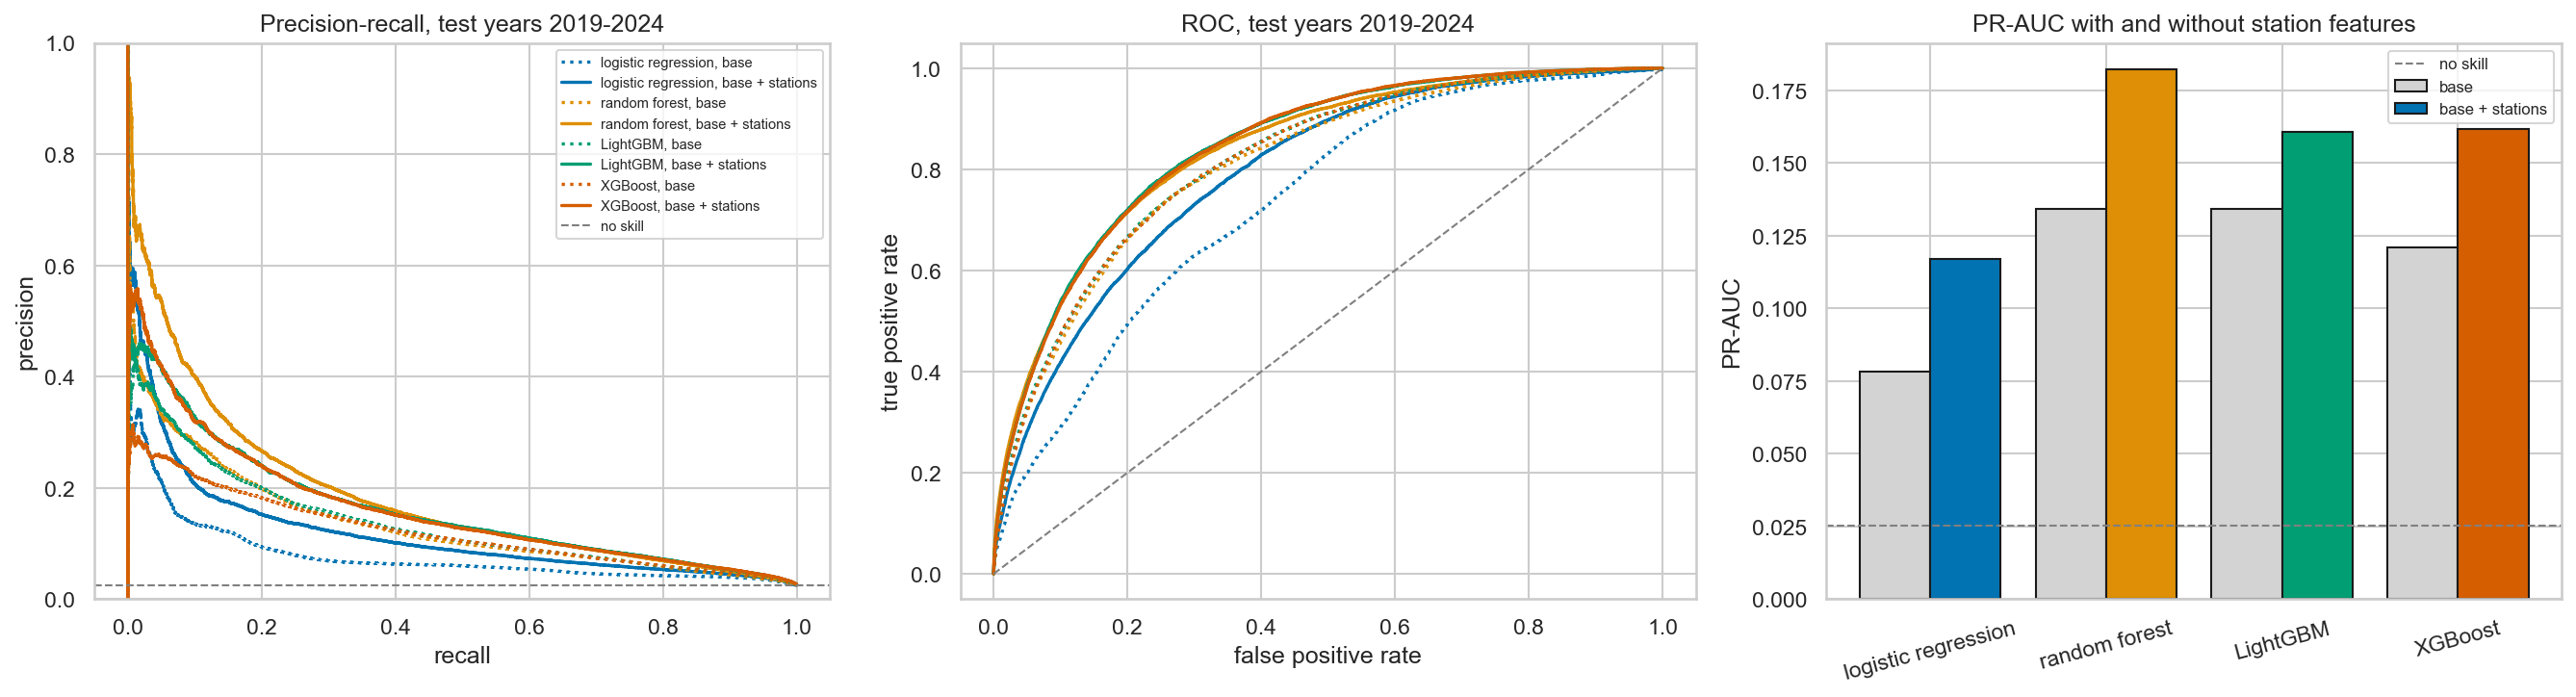
\includegraphics[width=\textwidth]{benchmark_curves.png}
\caption{Test years 2019--2024. Left: precision--recall curves (solid = with station features, dotted = base). Middle: ROC curves. Right: PR-AUC of each family without (grey) and with (colour) station features; the dashed line is the no-skill level.}
\label{fig:curves}
\end{figure*}

\subsection{Imbalance strategy}
Undersampling is best or tied for both families while training on a third of the rows (Table~\ref{tab:imbalance}), so every model below uses it. Full class weighting broke LightGBM (0.105): with positives weighted 33 times, validation PR-AUC peaks after a few rounds and early stopping ends training almost at once. The strategies mostly move the probability scale rather than the ranking: for the same logistic model the $F_1$-optimal threshold ranges from 0.095 to 0.764 while PR-AUC barely changes, which is why every threshold is re-chosen on validation data.

\begin{table}[!htb]
\centering\small
\caption{Imbalance strategies on the validation years (full feature set). $F_1$ at the $F_1$-optimal threshold.}
\label{tab:imbalance}
\begin{tabular}{@{}llccc@{}}
\toprule
Model & Strategy & PR-AUC & ROC-AUC & $F_1$ \\
\midrule
Logistic & none & 0.124 & 0.793 & 0.189 \\
Logistic & class weight & 0.126 & 0.801 & 0.195 \\
Logistic & \textbf{undersample 1:10} & \textbf{0.128} & 0.797 & \textbf{0.198} \\
\midrule
LightGBM & none & 0.240 & 0.862 & 0.301 \\
LightGBM & class weight & 0.105 & 0.797 & 0.175 \\
LightGBM & \textbf{undersample 1:10} & \textbf{0.249} & \textbf{0.864} & \textbf{0.311} \\
\bottomrule
\end{tabular}
\end{table}

\subsection{Model benchmark}
Station features improve every family (Table~\ref{tab:bench}, Figure~\ref{fig:curves}): PR-AUC rises from 0.078 to 0.117 for logistic regression, 0.134 to 0.182 for the random forest, 0.134 to 0.161 for LightGBM and 0.121 to 0.162 for XGBoost, and the tree models' ROC-AUC rises from 0.81--0.82 to 0.84--0.85. The random forest with stations is the best test model (PR-AUC 0.182, about $7\times$ no-skill; $F_1$ 0.242). The trees beat logistic regression by a wide margin because location, state and season interact non-linearly; logistic regression still gains the most in relative terms (+49\%), consistent with the roughly linear log-distance trend found in Milestone~1.

\begin{table}[!htb]
\centering\footnotesize
\setlength{\tabcolsep}{3.5pt}
\caption{Test-year results (2019--2024), with and without station features (``+st.''). Thresholds chosen on 2017--2018; no-skill PR-AUC = 0.025. LR = logistic regression, RF = random forest, LGBM = LightGBM, XGB = XGBoost. Best per column in bold.}
\label{tab:bench}
\begin{tabular}{@{}llcccccc@{}}
\toprule
Model & Set & Val PR & PR-AUC & ROC & $F_1$ & Prec. & Rec. \\
\midrule
LR & base & 0.093 & 0.078 & 0.735 & 0.134 & 0.109 & 0.172 \\
 & +st. & 0.128 & 0.117 & 0.794 & 0.175 & 0.124 & 0.293 \\
RF & base & 0.229 & 0.134 & 0.810 & 0.199 & 0.147 & 0.309 \\
 & +st. & 0.227 & \textbf{0.182} & 0.839 & \textbf{0.242} & \textbf{0.201} & 0.302 \\
LGBM & base & 0.236 & 0.134 & 0.818 & 0.206 & 0.162 & 0.284 \\
 & +st. & \textbf{0.249} & 0.161 & \textbf{0.845} & 0.228 & 0.172 & \textbf{0.337} \\
XGB & base & 0.228 & 0.121 & 0.817 & 0.200 & 0.146 & 0.315 \\
 & +st. & 0.248 & 0.162 & 0.844 & 0.229 & 0.179 & 0.316 \\
\bottomrule
\end{tabular}
\end{table}

\begin{figure*}[t]
\centering
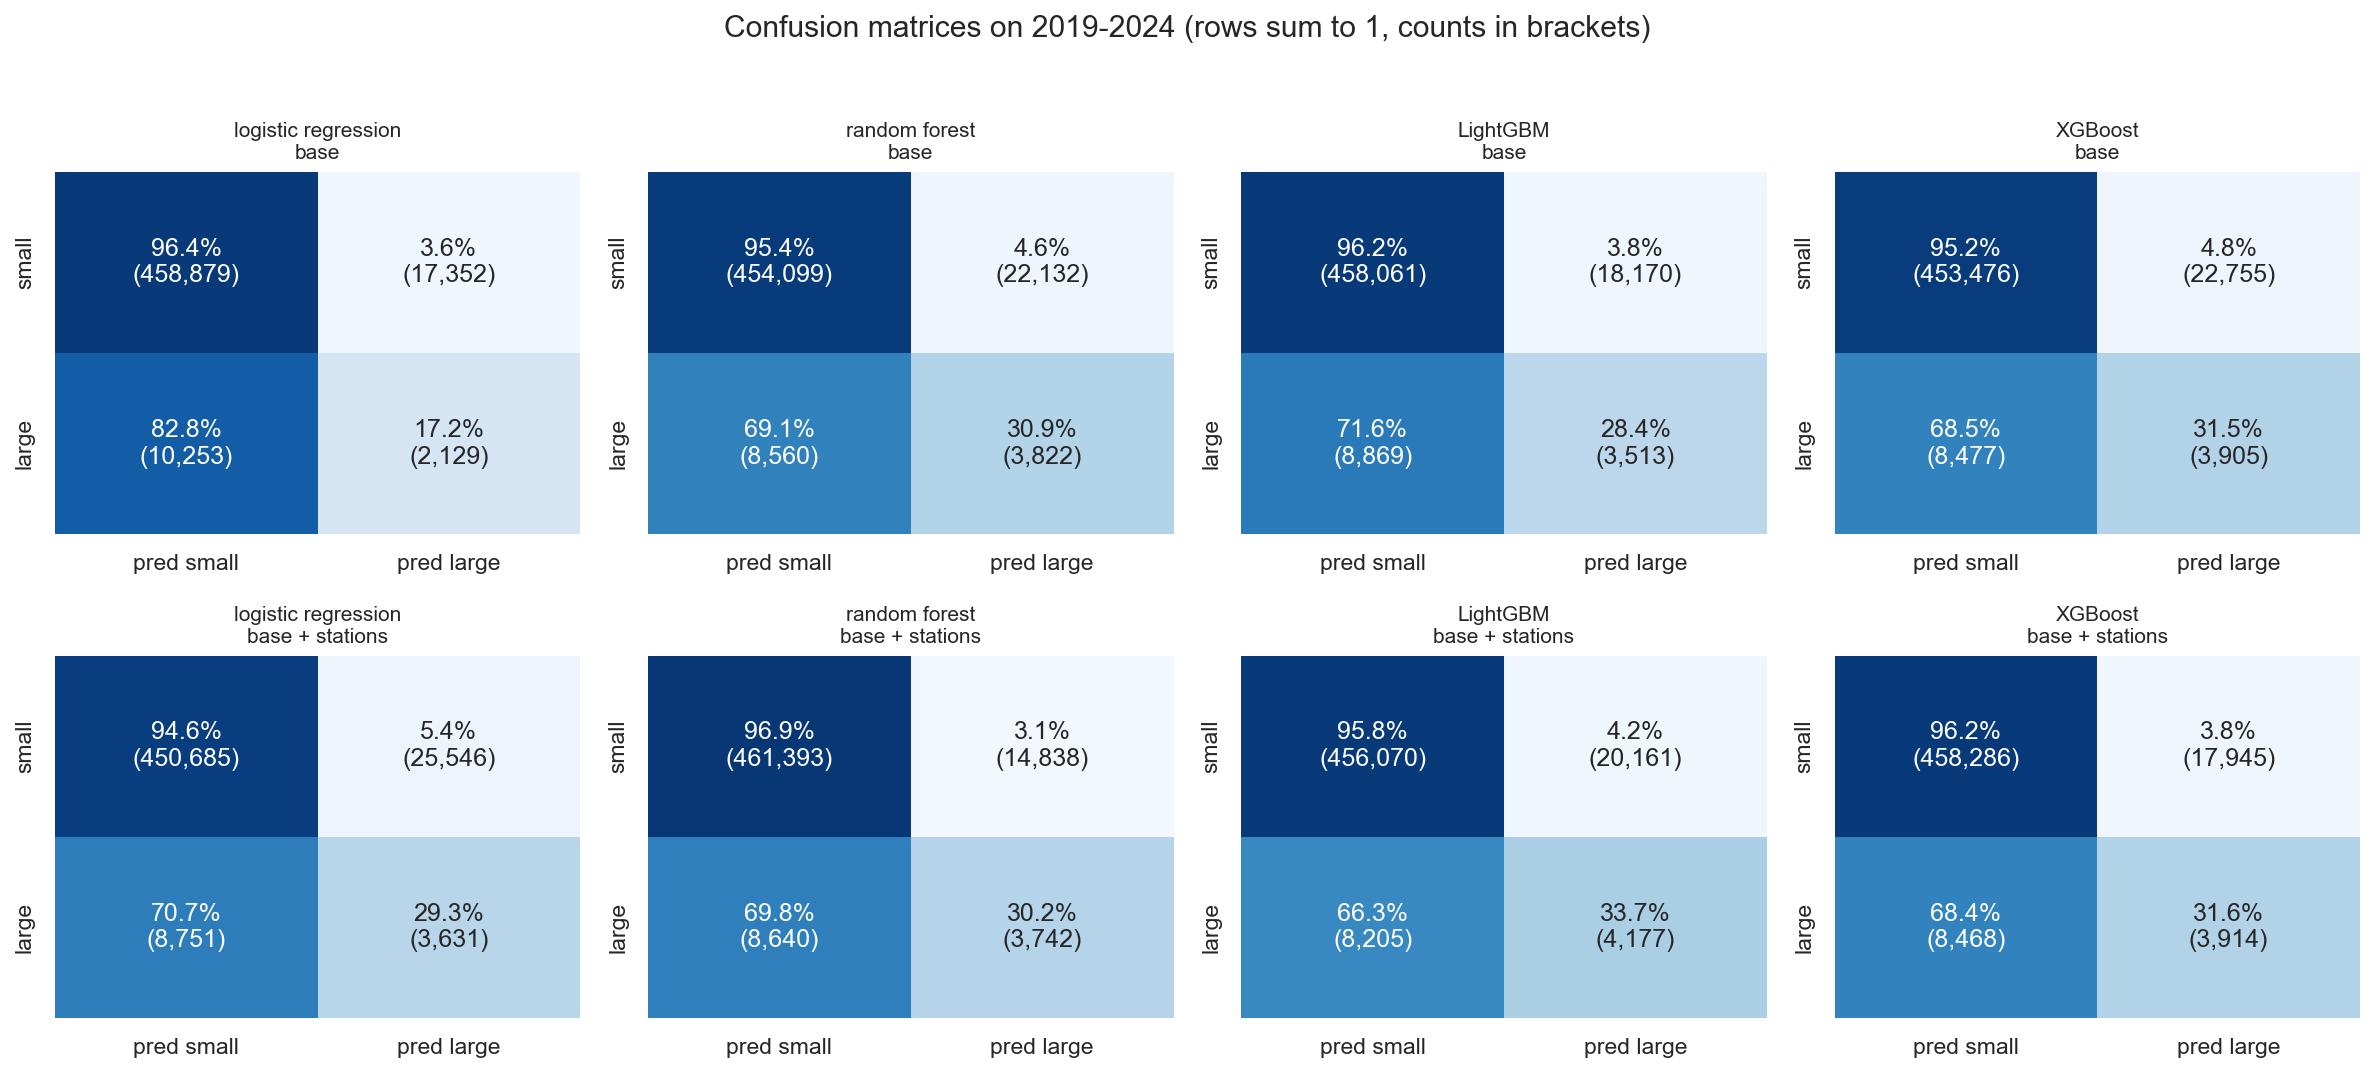
\includegraphics[width=0.88\textwidth]{confusion_matrices.png}
\caption{Row-normalised confusion matrices on 2019--2024 at each model's validation-chosen threshold (counts in brackets). Top row: base features; bottom row: with station features.}
\label{fig:cm}
\end{figure*}

\paragraph{Validation and test disagree.} Validation PR-AUC is about 0.25 against about 0.16 on test, and the ranking changes: the random forest is last on validation but first on test, and its station gain only appears on the test years. The test years have fewer large fires (2.5\% vs 3.1\%) and include the 2020--21 reporting changes, and the distance effect is stronger in recent years (Section~\ref{sec:effect}). A single two-year validation window is therefore a fragile basis for model selection, and the optimisation phase will use several time-blocked folds.

\paragraph{Confusion matrices.} At the $F_1$ threshold the tree models catch 30--34\% of large fires while flagging only 3--5\% of small fires (Figure~\ref{fig:cm}); roughly one flagged fire in five becomes large, against one in forty by chance. Adding station features to LightGBM raises recall from 28.4\% to 33.7\% at almost the same false-positive rate (3.8\% vs 4.2\%).

\begin{figure*}[t]
\centering
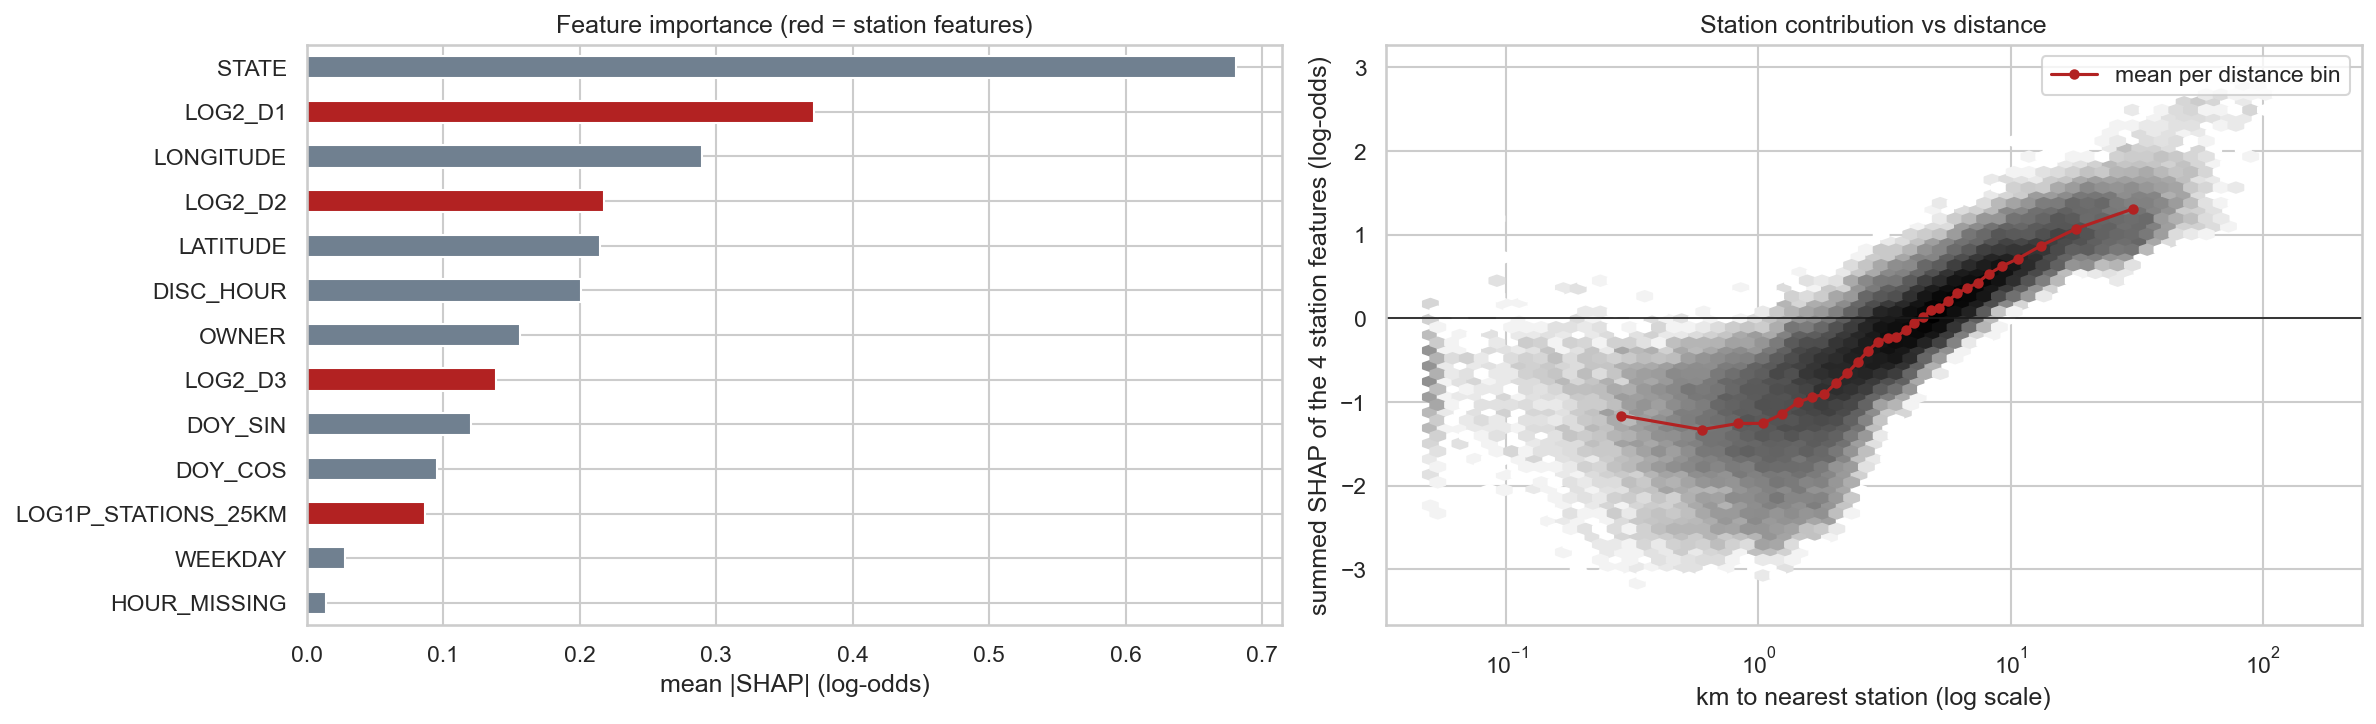
\includegraphics[width=\textwidth]{shap_distance.png}
\caption{LightGBM with station features, 100{,}000 test fires. Left: mean absolute SHAP value per feature (red = station features). Right: summed SHAP contribution of the four station features against distance to the nearest station (log scale); the red line is the mean in 30 equal-size distance bins.}
\label{fig:shap}
\end{figure*}

\subsection{Size and robustness of the station effect}
\label{sec:effect}
\paragraph{The gain is not noise.} Every block-bootstrap interval excludes zero (Table~\ref{tab:gain}), and in all 200 resamples the station features help all four families.

\begin{table}[!htb]
\centering\small
\caption{PR-AUC gain from the station features on the test years, with 95\% block-bootstrap intervals (315 state-year blocks, 200 resamples).}
\label{tab:gain}
\begin{tabular}{@{}lcc@{}}
\toprule
Model & Gain & 95\% interval \\
\midrule
Logistic regression & +0.039 & +0.028 to +0.052 \\
Random forest & +0.048 & +0.027 to +0.063 \\
LightGBM & +0.026 & +0.019 to +0.033 \\
XGBoost & +0.041 & +0.029 to +0.051 \\
\bottomrule
\end{tabular}
\end{table}

\paragraph{Distance is not a stand-in for cause.} Adding cause class to LightGBM \emph{lowers} test PR-AUC (0.134 to 0.120 without stations, 0.161 to 0.154 with them), as it did in Milestone~1, because the share of fires with a missing cause changes over time. With cause in the model the station features still add +0.034.

\paragraph{Effect size.} The adjusted training-year odds ratio, 1.78, matches the 1.80 found in Milestone~1 with a different model and sample (Table~\ref{tab:or}). Going from 2~km to 32~km (four doublings) multiplies the odds of a large fire by roughly $1.78^4\approx 10$. The effect is larger in 2019--2024 (2.08), which fits the station layer describing recent years best and means the test-year gain may be slightly flattering.

\begin{table}[!htb]
\centering\small
\caption{Odds ratio of a large fire per doubling of distance. ``Adjusted'' controls for state, land owner, season and year.}
\label{tab:or}
\begin{tabular}{@{}llcc@{}}
\toprule
Years & Model & OR & 95\% CI \\
\midrule
1992--2016 & unadjusted & 1.85 & 1.82--1.89 \\
1992--2016 & adjusted & \textbf{1.78} & 1.74--1.83 \\
2019--2024 & unadjusted & 2.25 & 2.21--2.30 \\
2019--2024 & adjusted & \textbf{2.08} & 2.03--2.14 \\
\bottomrule
\end{tabular}
\end{table}

\subsection{Localised evaluation}
The gain is positive in all eight regions (Table~\ref{tab:region}) and largest where stations are sparse and fires grow: Alaska (+0.103), the Plains (+0.033) and the Mountain West (+0.024). It is smallest in the Southeast and North/East (+0.007), where stations are dense and distance varies little. One national threshold behaves very differently across regions: recall is 92\% in Alaska and 55\% in the Plains but only 14--16\% in the Pacific, Southeast and North/East, so region-specific thresholds are a cheap improvement.

\begin{table}[!htb]
\centering\footnotesize
\setlength{\tabcolsep}{3.5pt}
\caption{LightGBM on the test years by region, sorted by prevalence. PR-AUC without and with station features; recall and precision at the single national threshold.}
\label{tab:region}
\begin{tabular}{@{}lccccrr@{}}
\toprule
Region & Prev. & Base & +st. & Gain & Rec. & Prec. \\
\midrule
Alaska & 20.1\% & 0.458 & 0.561 & +0.103 & 92\% & 41\% \\
Plains & 4.6\% & 0.154 & 0.187 & +0.033 & 55\% & 15\% \\
Southwest & 4.0\% & 0.140 & 0.159 & +0.019 & 21\% & 19\% \\
HI / PR & 3.4\% & 0.238 & 0.253 & +0.015 & 34\% & 30\% \\
Mountain W. & 3.1\% & 0.111 & 0.135 & +0.024 & 36\% & 15\% \\
Pacific & 2.4\% & 0.096 & 0.113 & +0.017 & 14\% & 21\% \\
Southeast & 2.2\% & 0.126 & 0.133 & +0.007 & 15\% & 21\% \\
North / East & 0.6\% & 0.072 & 0.079 & +0.007 & 16\% & 12\% \\
\bottomrule
\end{tabular}
\end{table}

\paragraph{Leave-one-region-out.} With a whole region held out, the station features raise PR-AUC in seven of eight regions (Figure~\ref{fig:loro}; Alaska +0.161, Plains +0.056, Mountain West +0.036), so the model learns a distance relationship that transfers to places it has never seen rather than memorising locations. Absolute PR-AUC falls when a region is unseen (Pacific 0.113 to 0.050), which shows how much the main model relies on knowing each place. The exception, Hawaii and Puerto Rico ($-0.152$), has only 68 large test fires and island geography unlike any training region; the North/East shows no gain (+0.001) at 0.6\% prevalence.

\begin{figure}[!htb]
\centering
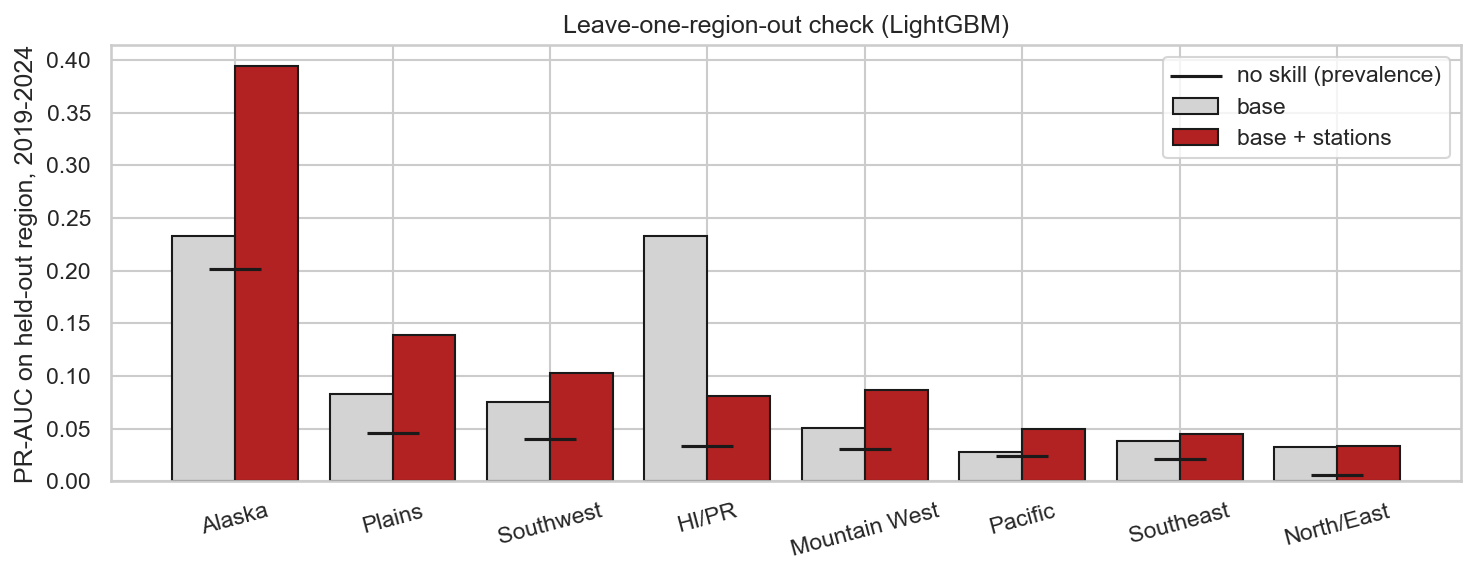
\includegraphics[width=\columnwidth]{spatial_holdout.png}
\caption{Leave-one-region-out check. LightGBM is trained on the 1992--2016 fires of all other regions (\code{STATE} dropped, undersampled 1:10, 400 trees) and scored on the 2019--2024 fires of the held-out region. Black ticks mark each region's no-skill level.}
\label{fig:loro}
\end{figure}

\subsection{What the model learned about distance}
Nearest-station distance is the second most important feature after \code{STATE}, and the four station features together contribute more than \code{STATE} (summed mean $|\text{SHAP}|$ about 0.81 against 0.68 log-odds; Figure~\ref{fig:shap}). The station contribution is flat below about 1~km, rises almost linearly in log distance after that, crosses zero near 4~km (the median fire) and keeps rising past 30~km. Between the nearest and farthest distance bins it changes the odds of a large fire by about $\times$12, in line with the odds ratio over the same range. The flat section suggests that within a kilometre, dispatch time rather than travel time limits the response.

%=====================================================================
\section{Discussion and Limitations}
%=====================================================================
\paragraph{Answer to RQ1 (preliminary).} Distance to the nearest fire station carries real, transferable information about whether a fire becomes large. Each doubling of distance raises the odds of a 100+ acre fire by about 1.8 times after adjustment (2.1 in 2019--2024), and adding station features to discovery-time models raises test PR-AUC in all four model families, in all eight regions, and in seven of eight regions unseen during training.

\begin{itemize}
\item \textbf{Modest absolute performance.} The best PR-AUC is 0.18 and most large fires are still missed. Final fire size depends heavily on weather, fuel and terrain, none of which is in the FPA-FOD.
\item \textbf{Unstable model selection.} Validation and test years disagree on the ranking of model families, so the ``best model'' label is provisional until time-blocked cross-validation is in place.
\item \textbf{Station data.} The layer is a recent snapshot of mostly structural stations; federal wildland crews are largely missing, and older fires are matched to today's stations. Milestone~1 showed that randomly missing stations bias the effect toward zero, but systematically missing wildland bases could bias it either way.
\item \textbf{Calibration.} Undersampling inflates predicted probabilities. Rankings and thresholds are valid, but the probabilities must be recalibrated before they are read as real risks.
\item \textbf{Small regions.} Alaska and Hawaii / Puerto Rico rest on a few hundred large fires and their numbers are noisy.
\end{itemize}

%=====================================================================
\section{Next Steps (Optimisation Phase)}
%=====================================================================
\begin{enumerate}
\item Tune LightGBM, XGBoost and the random forest with Optuna \cite{akiba2019} on expanding time-blocked folds inside 1992--2018, then refit on all of 1992--2018 before the final test.
\item Try milder class weights (for example $\times$5.8, the square root) and calibrate probabilities with isotonic regression on held-out years.
\item Choose region-specific thresholds.
\item Add engineered features computed only from earlier years: past fire density and large-fire rate per grid cell, and distance to wildland-agency stations.
\item Run a matched comparison of fires in the same cell, season and cause class at different distances, as a second estimate of the effect with fewer confounders.
\end{enumerate}

\paragraph{Reproducibility.} Data loading and the station join are in \code{src/features.py}, metric and imbalance helpers in \code{src/modeling.py}, and pinned package versions in \code{requirements.txt}. Paths are found relative to the repository and all random seeds are fixed (281). A full run takes about 25 minutes on a 22-core laptop.

\begin{thebibliography}{99}
\bibitem{short2026} K.~C. Short. \emph{Spatial wildfire occurrence data for the United States, 1992--2024 [FPA\_FOD\_20260615]}, 7th ed. USDA Forest Service Research Data Archive, Fort Collins, CO.
\bibitem{hifld} U.S. Geological Survey / DHS Homeland Infrastructure Foundation-Level Data (HIFLD). \emph{Fire and Emergency Medical Service (EMS) Stations}. Archived on DataLumos, project 239161. \url{https://www.datalumos.org/datalumos/project/239161}
\bibitem{breiman2001} L.~Breiman. Random forests. \emph{Machine Learning}, 45(1):5--32, 2001.
\bibitem{ke2017} G.~Ke et al. LightGBM: a highly efficient gradient boosting decision tree. In \emph{Advances in Neural Information Processing Systems}, 2017.
\bibitem{chen2016} T.~Chen and C.~Guestrin. XGBoost: a scalable tree boosting system. In \emph{Proceedings of KDD}, 2016.
\bibitem{saito2015} T.~Saito and M.~Rehmsmeier. The precision-recall plot is more informative than the ROC plot when evaluating binary classifiers on imbalanced datasets. \emph{PLoS ONE}, 10(3):e0118432, 2015.
\bibitem{lundberg2017} S.~M. Lundberg and S.-I. Lee. A unified approach to interpreting model predictions. In \emph{Advances in Neural Information Processing Systems}, 2017.
\bibitem{akiba2019} T.~Akiba et al. Optuna: a next-generation hyperparameter optimization framework. In \emph{Proceedings of KDD}, 2019.
\end{thebibliography}

\end{document}
